\documentclass[dvipsnames, notes]{beamer}

\usepackage[utf8]{inputenc}
\usepackage{url}
\usepackage{amssymb}
\usepackage{amsmath}
\usepackage{amsbsy}
\usepackage{mathbbol}
\usepackage{mathtools}

% Diagrams
\usepackage{tikz}

% Mathbb doesn't support digits
\usepackage{bbm}

% inference rules
\usepackage{mathpartir}

% Abbreviations
\newcommand{\lambdacalc}{$\lambda$-calculus}
\newcommand{\picalc}{$\pi$-calculus}
\newcommand{\Picalc}{$\pi$-Calculus}

% Typing rules
\newcommand{\stacked}[1]{\mprset{flushleft} \inferrule*{}{#1}}
\newcommand{\datatype}[2]{{\mprset{fraction={===}} \inferrule{#1}{#2}}}

\newcommand{\type}[1]{\textcolor{BlueViolet}{\operatorname{#1}}}
\newcommand{\constr}[1]{\textcolor{BurntOrange}{\operatorname{#1}}}
\newcommand{\func}[1]{\textcolor{OliveGreen}{\operatorname{#1}}}

% Constructors
\newcommand{\PO}{\constr{\mathbb{0}}}
\newcommand{\comp}[2]{#1 \; \constr{\parallel} \; #2}
\newcommand{\new}{\constr{\boldsymbol{\nu}} \;}
\newcommand{\send}[2]{#1 \; \constr{\langle} \; #2 \;\constr{\rangle} \;}
\newcommand{\sendp}[2]{#1 \; \constr{\langle} \; #2 \; \constr{\rangle} \; . \;}
\newcommand{\recv}[1]{#1 \; \constr{\mathbb{()}} \;}
\newcommand{\recvp}[2]{#1 \; \constr{(} \; #2 \; \constr{)} \; . \; }
\newcommand{\suc}{\constr{\scriptstyle 1+}}
\newcommand{\unit}{\constr{\mathbbm{1}}}
\newcommand{\base}[1]{\constr{B[} \; #1 \; \constr{]}}
\newcommand{\channel}[2]{\constr{C[} \; #1 \; \constr{;} \; #2 \; \constr{]}}
\newcommand{\comma}{\; \constr{,} \;}

% Functions
\newcommand{\subst}[3]{#1 \; \func{[} \; #3 \; \func{\mapsto} \;#2 \; \func{]}}
\newcommand{\op}[3]{#1 \; \func{\coloneqq} \; #2 \; \func{\cdot} \; #3}
\newcommand{\opsquared}[3]{#1 \, \func{\coloneqq} \, #2 \, \func{\cdot^2} \, #3}
\newcommand{\opctx}[3]{#1 \, \func{\coloneqq} \, #2 \, \func{\otimes} \, #3}
\newcommand{\zero}{\func{0\cdot}}
\newcommand{\one}{\func{1\cdot}}
\newcommand{\li}{\func{\ell_i}}
\newcommand{\lo}{\func{\ell_o}}
\newcommand{\lz}{\func{\ell_{\o}}}
\newcommand{\lio}{\func{\ell_{\#}}}

% Types
\newcommand{\Set}{\type{SET}}
\newcommand{\reduce}[1]{\; \type{\longrightarrow}_{#1} \;}
\newcommand{\types}[4]{#1 \; \type{;} \; #2 \; \type{\vdash} \; #3 \; \type{\triangleright} \; #4}
\newcommand{\contains}[6]{#1 \; \type{;} \; #2 \; \type{\ni}_{#3} \; #4 \; \type{;} \; #5 \; \type{\triangleright} \; #6}
\newcommand{\containsusage}[4]{#1 \; \type{\ni}_{#2} \; #3 \; \type{\triangleright} \; #4}
\newcommand{\Var}{\type{VAR}}
\newcommand{\Process}{\type{PROCESS}}
\newcommand{\Unused}{\type{UNUSED}}
\newcommand{\PreCtx}{\type{PRECTX}}
\newcommand{\Ctx}{\type{CTX}}
\newcommand{\Type}{\type{TYPE}\;}
\newcommand{\Idx}{\type{IDX}\;}
\newcommand{\Idxs}{\type{IDXS}}
\newcommand{\Usage}{\type{USAGE}}
\newcommand{\N}{\type{\mathbb{N}}}
\newcommand{\Channel}{\type{CHANNEL}}
\newcommand{\Rec}{\type{REC}}
\newcommand{\Algebra}{\type{ALGEBRA}}
\newcommand{\eq}[1]{\; \type{\simeq}_{#1} \;}
\newcommand{\eqeq}{\; \type{\cong} \;}

\usetheme[sectionpage=none,numbering=none]{metropolis}
\setbeamertemplate{title separator}{}
\date{}

\title{$\pi$ with leftovers: \\ a mechanisation in Agda}
\author{\textbf{Uma Zalakain} \ and \  Ornela Dardha \\ University of Glasgow}

\begin{document}
  \maketitle

  \note[itemize]{
  \item Please interrupt at any time
  }

  \begin{frame}{Motivation and Constraints}
    \centering
    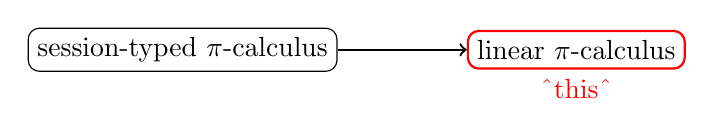
\begin{tikzpicture}
      \node[draw, rounded corners] (st) at (0,0) {session-typed \picalc{}};
      \node[draw=red, thick, rounded corners, label={[red]below:\textasciicircum this\textasciicircum}] (sh) at (5,0) {linear \picalc{}};
      \draw[->, thick] (st) -- (sh);
    \end{tikzpicture}
    \vspace{2em}

    \begin{itemize}
      \item Syntax and semantics must be untyped
      \item Must also support shared channels
      \item Goal: to prove subject reduction
    \end{itemize}
  \end{frame}

  \begin{frame}{Notation}
    \begin{equation*}
      \begin{aligned}
        & \type{TYPES}          && \text{blue violet, uppercased, indices as subscripts} \\
        & \constr{constructors} && \text{burnt orange} \\
        & \func{functions}      && \text{olive green} \\
        & variables             && \text{black, in italics} \\
      \end{aligned}
    \end{equation*}
  \end{frame}

  \note[itemize]{
  \item We want to encode the session-typed \picalc{} into the linear \picalc{}
  \item and prove some properties of the encoding
  \item We first need our target language: the linear \picalc{}
  \item Common syntax and semantics for linear and session-typed
  }
  
  \begin{frame}{\Picalc{}: Well-Scoped Syntax}
    \begin{mathpar}
      \inferrule
      {n : \N}
      {\constr{0} : \Var_{\suc n}}

      \inferrule
      {x : \Var_n}
      {\suc x : \Var_{\suc n}}
    \end{mathpar}

    \begin{equation*}
      \begin{aligned}
        \Process_n ::=& \; \PO_n               &&\text{(inaction)}    \\ 
        |& \; \new{} \Process_{\suc n}         &&\text{(restriction)} \\ 
        |& \; \comp{\Process_n}{\Process_n}    &&\text{(parallel)}     \\ 
        |& \; \recv{\Var_n}{}\Process_{\suc n} &&\text{(input)}       \\ 
        |& \; \send{\Var_n}{\Var_n}\Process_n  &&\text{(output)}       \\           
      \end{aligned}
    \end{equation*}
  \end{frame}

  \note[itemize]{
    \item \picalc{} syntax, well-scoped by construction through de Bruijn indices
    \item go over the constructors
  }

  \begin{frame}{\Picalc{}: Structural Congruence}
    \begin{mathpar}
      \inferrule
      { }
      {\constr{comp-assoc} : \comp{P}{(\comp{Q}{R})} \eqeq \comp{(\comp{P}{Q})}{R}}

      \inferrule
      { }
      {\constr{comp-sym} : \comp{P}{Q} \eqeq \comp{Q}{P}}
      
      \inferrule
      { }
      {\constr{comp-end} : \comp{P}{\PO_n} \eqeq P}
      
      \inferrule
      { }
      {\constr{scope-end} : \new \PO_{\suc n} \eqeq \PO_n}
      
      \inferrule
      {uQ : \Unused_{\constr{0}} \; Q}
      {\constr{scope-ext} : \new (\comp{P}{Q}) \eqeq \comp{(\new P)}{\func{lower}_{\constr{0}} \; \; Q \; uQ}}

      \inferrule
      { }
      {\constr{scope-comm} : \new \new P \eqeq \new \new \func{swap}_{\constr{0}} \; P}
    \end{mathpar}

    \centering
    $\eq{}$ is the congruent equivalence closure of $\eqeq$
  \end{frame}

  \note[itemize]{
    \item Parallel composition is associative, commutative and has $\PO$ as neutral element
    \item Garbage collection
    \item Scope extrusion (keep a proof $uQ$ alongside)
    \item Commutativity of scopes
  }

  \begin{frame}{\Picalc{}: Reduction Relation}
    \begin{mathpar}
      \inferrule
      { }
      {\constr{internal} : \Channel_n}

      \inferrule
      {i : \Var_n}
      {\constr{external} \; i : \Channel_n}

      \inferrule
      {i \; j : \Var_n \\ P : \Process_{\suc n} \\ Q : \Process_n}
      {\constr{comm} : \comp{\recv{i}P}{\send{i}{j}{Q}} \reduce{\constr{external} \; i} \comp{\func{lower}_{\constr{0}} \; (\subst{P}{\suc j}{\constr{0}}) \; uP'}{Q}}

      \inferrule
      {red : P \reduce{c} P'}
      {\constr{par} \; red : \comp{P}{Q} \reduce{c} \comp{P'}{Q}}

      \inferrule
      {red : P \reduce{c} Q}
      {\constr{res} \; red : \new P \reduce{\func{dec}\; c} \new Q}

      \inferrule
      {eq : P \eq{} P' \\ red : P' \reduce{c} Q}
      {\constr{struct} \; eq \; red : P \reduce{c} Q}
    \end{mathpar}
  \end{frame}

  \note[itemize]{
    \item Same scope before and after reduction
    \item Scope restriction is preserved (can be eliminated in strictly linear systems)
    \item Common channel $i$
    \item We keep track of $i$ at the type level
    \item Goes under parallel composition and scope restriction
    \item $\func{dec}$ saturates on $\constr{internal}$
  }

  \begin{frame}{Type System: Initial Pitfalls}
    \begin{itemize}
    \item Transforming contexts using functions
      \begin{mathpar}
      \inferrule
      {\stacked{
          \gamma \; \type{;} \; \Gamma \; \type{\ni}_i \; \channel{t}{u} \; \type{;} \; x\\
          \opsquared{x}{\li}{z} \\\\
          \gamma \comma t \; \type{;} \; (\func{update}_i \; z \; \Gamma) \comma u \vdash P}}
      {\gamma \; \type{;} \; \Gamma \; \type{\vdash} \; \recv{i}{P}}
      \end{mathpar}
    \item Extrinsic context splits
      \begin{mathpar}
        \inferrule
        {\stacked{
            \opctx{\Gamma}{\Delta}{\Xi} \\\\
            \gamma \; \type{;} \; \Delta \; \type{\vdash} P \\\\
            \gamma \; \type{;} \; \Xi \; \type{\vdash} Q}}
        {\gamma \; \type{;} \; \Gamma \; \type{\vdash} \; \comp{P}{Q}}
      \end{mathpar}
    \end{itemize}
  \end{frame}

  \begin{frame}{Type System}
    \begin{itemize}
      \item Syntax directed
      \item Intrinsic context splits
      \item Based on a set of usage algebras
    \end{itemize}
  \end{frame}
  
  \note[itemize]{
  \item Top down
  \item Only choice is in the types and usage annotations on scope restriction
  }

  \begin{frame}{Usage Algebra}
    \begin{equation*}
    \begin{aligned}
      &\zero                 &:{} &                 &        & C \\
      &\one                  &:{} &                 &        & C \\
      &\op{\_}{\_}{\_}       &:{} &                 &        & C \to C \to C \to \Set \\
      &\func{\cdot-compute}  &:{} &\forall y z       & \to \; & \type{DEC} \; (\type{\exists} x  \; (\op{x}{y}{z})) \\
      &\func{\cdot-unique}   &:{} &\forall x x' y z  & \to \; & \op{x'}{y}{z} \to \op{x}{y}{z} \to x' \equiv x \\
      &\func{\cdot-unique^l} &:{} &\forall x y y' z  & \to \; & \op{x}{y'}{z} \to \op{x}{y}{z} \to y' \equiv y \\
      &\func{\cdot-min^l}    &:{} &\forall y z        & \to \; & \op{\zero}{y}{z} \to y \equiv \zero \\
      &\func{\cdot-id^l}     &:{} &\forall x         & \to \; & \op{x}{\zero}{x} \\
      &\func{\cdot-comm}     &:{} &\forall x y z     & \to \; & \op{x}{y}{z} \to \op{x}{z}{y} \\
      &\func{\cdot-assoc}    &:{} &\forall x y z u v & \to \; & \op{x}{y}{z} \to \op{y}{u}{v} \to \\
      &                      &    &                  &        & \type{\exists} w  \; (\op{x}{u}{w} \times \op{w}{v}{z})
    \end{aligned}
    \end{equation*}
  \end{frame}

  \note[itemize]{
    \item Model as a ternary relation
    \item Decidable, deterministic, cancellative and has a minimal element
  }

  \begin{frame}{Notation}
    \begin{equation*}
      \begin{aligned}
        &C^{\func{2}} &&= C \type{\times} C \\
        &\lz          &&= \zero \comma \zero \\
        &\li          &&= \one \comma \zero \\
        &\lo          &&= \zero \comma \one \\
        &\lio         &&= \one \comma \one \\
        &\opsquared{(x_l \comma x_r)}{(y_l \comma y_r)}{(z_l \comma z_r)} &&= (\op{x_l}{y_l}{z_l}) \times (\op{x_r}{y_r}{z_r}) \\
      \end{aligned}
    \end{equation*}
  \end{frame}
  
  \begin{frame}{Indexed Usage Algebras}
    \begin{equation*}
      \begin{aligned}
        &\Idx               &:{} &\Set \\
        &\type{\exists IDX} &:{} &\Idx \\
        &\Usage             &:{} &\Idx \to \Set \\
        &\type{ALGEBRAS}    &:{} &(idx : \Idx) \to \Algebra_{\Usage_{idx}} \\
      \end{aligned}
    \end{equation*}
  \end{frame}

  \note[itemize]{
    \item Lump multiple algebras together
  }
  
  \begin{frame}{Typing Contexts}
    \begin{mathpar}
      \inferrule
      { }
      {\unit : \Type}

      \inferrule
      {n : \N}
      {\base{n} : \Type}
      
      \inferrule
      {t : \Type \\ \stacked{idx : \Idx \\\\ x : \Usage_{idx}^{\func{2}}}}
      {\channel{t}{x} : \Type}
      
      \inferrule
      { }
      {[] : \PreCtx_{\constr{0}}}
      
      \inferrule
      {\gamma : \PreCtx_n \\ t : \Type}
      {\gamma \comma t : \PreCtx_{\suc n}}
    \end{mathpar}
  \end{frame}

  \begin{frame}{Usage Contexts}
    \begin{mathpar}
      \inferrule
      { }
      {[] : \Idxs_{\constr{0}}}
      
      \inferrule
      {idxs : \Idxs_n \\ idx : \Idx}
      {idxs \comma idx : \Idxs_{\suc n}} \\
      
      \inferrule
      { }
      {[] : \Ctx_{[]}}
      
      \inferrule
      {\Gamma : \Ctx_{idxs} \\ x : \Usage_{idx} ^{\func{2}}}
      {\Gamma \comma x : \Ctx_{idxs \comma idx}}
    \end{mathpar}
  \end{frame}

  \note[itemize]{
  \item Usage context independent of typing contexts
  }

  \begin{frame}{Type System}
    \tiny
    \begin{mathpar}
    \datatype{
      \gamma : \PreCtx_n \\
      \stacked{
        idxs : \Idxs_n \\\\
        \Gamma : \Ctx_{idxs}} \\
      i : \Var_n \\
      t : \Type \\
      \stacked{
        idx : \Idx \\\\
        y : \Usage_{idx}^{\func{2}}} \\
      \Delta : \Ctx_{idxs}}
    {\contains{\gamma}{\Gamma}{i}{t}{y}{\Delta} : \Set}
    \; \textsc{VarRef}

    \datatype{
      \gamma : \PreCtx_n \\
      \stacked{
        idxs : \Idxs_n \\\\
        \Gamma : \Ctx_{idxs}} \\
      P : \Process_n \\
      \Delta : \Ctx_{idxs}}
    {\types{\gamma}{\Gamma}{P}{\Delta} : \Set}
    \; \textsc{Types}
    \end{mathpar}
  \end{frame}
  
  \begin{frame}{Variable References}
    \begin{mathpar}
      \inferrule
      {\opsquared{x}{y}{z}}
      {\constr{0} : \contains{\gamma \comma t}{\Gamma \comma x}{\constr{0}}{t}{y}{\Gamma \comma z}}
      
      \inferrule
      {\hspace{-0.1em} loc_i : \contains{\gamma \hspace{1.4em}}{\Gamma \hspace{1.7em}}{\hspace{1em} i}{t}{x}{\Delta}}
      {\suc \; loc_i : \contains{\gamma \comma t'}{\Gamma \comma x'}{\suc i}{t}{x}{\Delta \comma x'}}
    \end{mathpar}
  \end{frame}

  \note[itemize]{
  \item Constructor completely determined by $i$
  \item User alleviated from proof burden $\opsquared{x}{y}{z}$, which can be computed given $x$ and $y$
  }
  
  \begin{frame}{Typing Rules}
    \begin{mathpar}
    \inferrule
    { }
    {\constr{end} : \types{\gamma}{\Gamma}{\PO}{\Gamma}}
  
    \inferrule
    {t : \Type \\ x : \Usage_{idx}^{\func{2}} \\ y : \Usage_{idx'} \\\\
     cont : \types{\gamma \comma \channel{t}{x}}{\Gamma \comma (y \comma y) }{P}{\Delta \comma \lz}}
    {\constr{chan} \; t \; x \; y \; cont : \types{\gamma}{\Gamma}{\new P}{\Delta}}
    \end{mathpar}
  \end{frame}
  
  \begin{frame}{Typing Rules}
    \begin{mathpar}
    \inferrule
        {\stacked{
            chan_i : \contains{\gamma \hspace{1.2em}}{\Gamma \hspace{1.5em}}{i}{\channel{t}{x}}{\li}{\Xi} \\\\
            cont \hspace{0.4em} : \types{\gamma \comma t}{\Xi \comma x}{P \hspace{4.6em}}{\Theta \comma \lz}}}
        {\constr{recv} \; chan_i \; cont : \types{\gamma}{\Gamma}{\recv{i}{P}}{\Theta}}
  
    \inferrule
        {\stacked{
            chan_i : \contains{\gamma}{\Gamma \hspace{0.2em}}{i}{\channel{t}{x}}{\lo}{\Delta} \\\\
            loc_j \hspace{0.7em} : \contains{\gamma}{\Delta}{j}{t \hspace{3.1em}}{x \hspace{0.3em}}{\Xi} \\\\
            cont \hspace{0.3em} : \types{\gamma}{\Xi \hspace{0.3em}}{P\hspace{4.8em}}{\Theta}}}
        {\constr{send} \; chan_i \; loc_j \; cont : \types{\gamma}{\Gamma}{\send{i}{j}P}{\Theta}}
  
    \inferrule
    {l \hspace{0.2em} : \types{\gamma}{\Gamma \hspace{0.3em}}{P}{\Delta} \\\\
     r : \types{\gamma}{\Delta}{Q}{\Xi}}
    {\constr{comp} \; l \; r : \types{\gamma}{\Gamma}{\comp{P}{Q}}{\Xi}}
    \end{mathpar}
  \end{frame}

  \note[itemize]{
  \item Newly introduced channels are balanced
  }

  \begin{frame}{Type Safety: auxiliary lemmas}
    \begin{itemize}
      \item Framing
      \item Weakening
      \item Strengthening
      \item Swapping
    \end{itemize}
  \end{frame}

  \begin{frame}{Type Safety: subject congruence}
  \end{frame}

  \begin{frame}{Type Safety: substitution}
  \end{frame}

  \begin{frame}{Type Safety: subject reduction}
  \end{frame}

  \begin{frame}{Future Work}
    \begin{itemize}
    \item Prove preservation of balancedness
    \item Product and sum types
    \item Recursion
    \item Bidirectional type system
    \item Decidable type checking
    \item Encoding session types into it
    \end{itemize}
  \end{frame}
\end{document}